%\documentclass[usenames,dvipsnames,12pt,handout]{beamer}
\documentclass[usenames,dvipsnames,12pt]{beamer}

\usecolortheme{dove}
\usefonttheme{professionalfonts}
\usefonttheme{serif}

\usepackage{bm}
\usepackage{mathtools}
\usepackage{amsmath,amssymb,amsfonts,amsthm}
\usepackage{mathrsfs}
\usepackage{mathabx}
\usepackage{fontspec}
\usepackage{multicol}
\usepackage{xcolor}
\usepackage{pifont}
\usepackage{tabularx}
\usepackage{colortbl}
\usepackage{graphicx}
\usepackage{semantic}
\usepackage{xspace}
\usepackage[all]{xy}
\usepackage{listings}
\usepackage{lstautogobble}
\usepackage{fancybox}
\usepackage{stmaryrd}
\usepackage{rotating}
\usepackage{wasysym}
\usepackage{ulem}
\usepackage{soul}
\usepackage{newunicodechar}
\usepackage[super]{nth}
\usepackage{tikz, tikz-qtree, tikz-qtree-compat}
\usetikzlibrary{shapes, arrows, calc, quotes, tikzmark, decorations.pathreplacing, decorations.markings}
\usepackage{makecell}
\usepackage{epigraph}

\hypersetup{colorlinks=true,linkcolor=Cyan,urlcolor=Cyan,citecolor=Cyan}

\setlength{\multicolsep}{3pt}
\setlength{\columnseprule}{0.5pt}

\newcommand\mytikzmark[2]{\tikz[overlay,remember picture, anchor=base] \node (#1) {#2};}

% colored underline, with Beamer overlay support
% usage: \cul{x} or \cul[blue]{x} or \cul<2->{x} or \cul<2->[blue]{x}
\newcommand<>{\cul}[2][Red]{
  \fontdimen8\textfont3=0.75pt
  \alt#3
      {\color{#1}\underline{{\color{black}#2}}\color{black}}
      {\transparent{0.0}\underline{{\transparent{1.0}#2}}\transparent{1.0}}
}
\newcommand{\smalltt}[1]{{\small \texttt{#1}}}
\newcommand{\McL}{\mathscr{L}}
\newcommand{\yes}{\textcolor{Green}{\ding{51}}}
\newcommand{\no}{\textcolor{Red}{\ding{55}}}
\newcommand{\maybe}{\ding{82}}
\newcommand{\redtext}[1]{\textcolor{Maroon}{#1}}
\newcommand{\bluetext}[1]{\textcolor{NavyBlue}{#1}}
\newcommand{\orangetext}[1]{\textcolor{BurntOrange}{#1}}
\newcommand{\greentext}[1]{\textcolor{PineGreen}{#1}}
\newcommand{\graytext}[1]{\textcolor{gray}{#1}}
\newcommand{\purpletext}[1]{\textcolor{Plum}{#1}}
\newcommand{\bl}[1]{\ensuremath{\orangetext{#1}}}
\newcommand{\key}[1]{\ensuremath{\mathtt{#1}}}
\newcommand{\MID}{\;\mid\;}
\newcommand{\Surface}{\ensuremath{\lambda_{\mathtt{IFC}}^\star}\xspace}
\newcommand{\SurfaceOld}{\ensuremath{\lambda_{\mathtt{SEC}}^\star}\xspace}
\newcommand{\CCOld}{\ensuremath{\lambda_{\mathtt{SEC}}^{\Rightarrow}}\xspace}
\newcommand{\CC}{\ensuremath{\lambda_{\mathtt{IFC}}^{c}}\xspace}
\newcommand{\GSLRef}{\ensuremath{\mathrm{GSL}_\mathsf{Ref}}\xspace}
\newcommand{\GSLRefEps}{\ensuremath{\mathrm{GSL}_\mathsf{Ref}^\epsilon}\xspace}
\newcommand{\SSLRef}{\ensuremath{\mathrm{SSL}_\mathsf{Ref}}\xspace}
\newcommand{\lamgif}{\ensuremath{\mathit{\lambda_{gif}}}\xspace}
\newcommand{\WHILEG}{WHILE\textsuperscript{G}\xspace}
\newcommand{\high}{\textcolor{OrangeRed}{\key{high}}\xspace}
\newcommand{\low}{\textcolor{PineGreen}{\key{low}}\xspace}
\newcommand{\unk}{\textcolor{Maroon}{\key{\star}}\xspace}
\newcommand{\Bool}{\key{Bool}}
\newcommand{\Int}{\key{Int}}
\newcommand{\Unit}{\key{Unit}}
\newcommand{\Fun}[3]{\ensuremath{{#1}\xrightarrow{{#2}}{#3}}}
\newcommand{\Refer}[1]{\ensuremath{\key{Ref}\;{#1}}}
\newcommand{\true}{\key{true}}
\newcommand{\false}{\key{false}}
\newcommand{\unit}{\key{unit}}
\newcommand{\pc}{\ensuremath{\mathit{pc}}\xspace}
\newcommand{\PC}{\ensuremath{\mathit{PC}}\xspace}
\newcommand{\gc}{\ensuremath{\mathit{gc}}\xspace}
\newcommand{\syntax}[1]{\text{\texttt{\textcolor{Purple}{#1}}}}
\newcommand{\ccsyntax}[1]{\text{\texttt{{#1}}}}
\newcommand{\const}[2]{\ensuremath{\syntax{(\$}\;{#1}\syntax{)}_{#2}}}
\newcommand{\lam}[5]{\ensuremath{\syntax{(λ}^{#1}{#2}\syntax{:}{#3}\syntax{.}\,{#4}\syntax{)}_{#5}}}
\newcommand{\app}[3]{\ensuremath{\syntax{(}{#1}\;{#2}\syntax{)}^{\bl{#3}}}}
\newcommand{\ifexp}[4]{\ensuremath{\syntax{(if}\;{#1}\;\syntax{then}\;{#2}\;\syntax{else}\;{#3}\syntax{)}^{\bl{#4}}}}
\newcommand{\refexp}[3]{\ensuremath{\syntax{(ref}\;{#1}\;{#2}\syntax{)}^{\bl{#3}}}}
\newcommand{\deref}[2]{\ensuremath{\syntax{!}^{\bl{#2}}\;{#1}}}
\newcommand{\assign}[3]{\ensuremath{\syntax{(}{#1}\;\syntax{:=}\;{#2}\syntax{)}^{\bl{#3}}}}
\newcommand{\ann}[3]{\ensuremath{\syntax{(}{#1}\;\syntax{:}\;{#2}\syntax{)}^{\bl{#3}}}}
\newcommand{\letexp}[3]{\ensuremath{\syntax{let}\;{#1}={#2}\;\syntax{in}\;{#3}}}
\newcommand{\ccconst}[1]{\ensuremath{\ccsyntax{\$}\;{#1}}}
\newcommand{\ccaddr}[1]{\ensuremath{\ccsyntax{addr}\;{#1}}}
\newcommand{\cclam}[2]{\ensuremath{\ccsyntax{λ}{#1}\ccsyntax{.}\,{#2}}}
\newcommand{\ccif}[5]{\ensuremath{\ccsyntax{if}\;{#1}\;{#2}\;{#3}\;{#4}\;{#5}}}
\newcommand{\ccifstar}[4]{\ensuremath{\ccsyntax{if}{\star}\,{#1}\,{#2}\,{#3}\,{#4}}}
\newcommand{\ccref}[2]{\ensuremath{\ccsyntax{ref}\;{#1}\;{#2}}}
\newcommand{\ccrefproj}[3]{\ensuremath{\ccsyntax{ref?}^{\bl{#3}}\;{#1}\;{#2}}}
\newcommand{\ccderef}[3]{\ensuremath{\ccsyntax{!}\;{#1}\;{#2}\;{#3}}}
\newcommand{\ccderefstar}[2]{\ensuremath{\ccsyntax{!}{\star}\,{#1}\,{#2}}}
\newcommand{\ccassign}[5]{\ensuremath{\ccsyntax{assign}\;{#1}\;{#2}\;{#3}\;{#4}\;{#5}}}
\newcommand{\ccassignproj}[5]{\ensuremath{\ccsyntax{assign?}^{\bl{#5}}\;{#1}\;{#2}\;{#3}\;{#4}}}
\newcommand{\cccast}[2]{\ensuremath{{#1}\,\ccsyntax{⟨}\,{#2}\,\ccsyntax{⟩}}}
\newcommand{\ccprot}[4]{\ensuremath{\ccsyntax{prot}\;{#1}\;{#2}\;{#3}\;{#4}}}
\newcommand{\cccastpc}[2]{\ensuremath{\ccsyntax{cast}_{\ccsyntax{pc}}\;{#1}\;{#2}}}
\newcommand{\cclet}[4]{\ensuremath{\ccsyntax{let}\;{#1}\ccsyntax{=}{#2}\ccsyntax{:}{#3}\;\ccsyntax{in}\;{#4}}}
\newcommand{\ccapp}[5]{\ensuremath{\ccsyntax{app}\;{#1}\;{#2}\;{#3}\;{#4}\;{#5}}}
\newcommand{\ccappstar}[4]{\ensuremath{\ccsyntax{app}{\star}\,{#1}\,{#2}\,{#3}\,{#4}}}
\newcommand{\ccopaque}{\ensuremath{\ccsyntax{●}}}
\newcommand{\lconsisjoin}{\ensuremath{\,\widetilde{\curlyvee}\,}}  % label consistent join
\newcommand{\consisjoin}{\ensuremath{\,\widetilde{\vee}\,}}        % type consistent join
\newcommand{\lconsismeet}{\ensuremath{\,\widetilde{\curlywedge}\,}}  % label consistent meet
\newcommand{\consismeet}{\ensuremath{\,\widetilde{\wedge}\,}}        % type consistent meet
\newcommand{\Cast}[3]{\ensuremath{{#1}\Rightarrow^{\bl{#3}}{#2}}}
\newcommand{\Type}{\textit{Type}}
\newcommand{\RawType}{\textit{RawType}}
\newcommand{\Label}{\textit{Label}}
\newcommand{\compile}[1]{\ensuremath{\mathcal{C}\;{#1}}}
\newcommand{\applycast}[3]{\ensuremath{\mathbf{Cast}\;{#1}\,,\,{#2}\leadsto{#3}}}
\newcommand{\blame}[1]{\ensuremath{\key{blame}\;\bl{#1}}}
\newcommand{\reduce}[5]{\ensuremath{{#1}\mid{#2}\mid{#3}\longrightarrow{#4}\mid{#5}}}
\newcommand{\Active}[1]{\ensuremath{\mathbf{Active}\;{#1}}}
\newcommand{\Inert}[1]{\ensuremath{\mathbf{Inert}\;{#1}}}
\newcommand{\bigstep}[5]{\ensuremath{{#1}\mid{#2}\vdash{#3}\Downarrow{#4}\mid{#5}}}
\newcommand{\bigstepe}[5]{\ensuremath{{#1}\mid{#2}\vdash{#3}\Downarrow_\epsilon{#4}\mid{#5}}}
%% coercions
\newcommand{\id}[1]{\ensuremath{\mathit{\bold{id}}(#1)}}
\newcommand{\up}{\ensuremath{\boldsymbol{\uparrow}}}
\newcommand{\inj}[1]{\ensuremath{{#1}\,\boldsymbol{!}}}
\newcommand{\seq}{\ensuremath{\,\boldsymbol{;}\,}}
\newcommand{\err}[3]{\ensuremath{\boldsymbol{\bot}^{\bl{#3}}\;{#1}\;{#2}}}
\newcommand{\proj}[2]{\ensuremath{{#1}\,\boldsymbol{?}^{\bl{#2}}}}
\newcommand{\coerc}[2]{\ensuremath{{#1}\boldsymbol{,}\,{#2}}}
\newcommand{\refco}[2]{\ensuremath{\mathbf{Ref}\;{#1}\;{#2}}}
\newcommand{\funco}[3]{\ensuremath{{#1}\boldsymbol{,}\,{#2}\boldsymbol{\rightarrow}{#3}}}
\newcommand{\precctx}[8]{\ensuremath{{#1};{#2};{#3};{#4};{#5};{#6};{#7};{#8}}}
\newcommand{\ccprec}[4]{\ensuremath{\vdash{#1}\sqsubseteq{#2}\Leftarrow{#3}\sqsubseteq{#4}}}

\newcommand{\highlight}[2]{\colorbox{#1}{\ensuremath{#2}}}
\newcommand{\highlightblue}[1]{\highlight{White!90!NavyBlue}{#1}}
\newcommand{\highlightred}[1]{\highlight{White!90!Maroon}{#1}}

\definecolor{highlight}{gray}{0.9}
\sethlcolor{highlight}

\newunicodechar{ℒ}{\ensuremath{\McL}}
\newunicodechar{𝕋}{\ensuremath{\mathbb{T}}}
\newunicodechar{𝕊}{\ensuremath{\mathbb{S}}}

\newtheorem{conjecture}[theorem]{\translate{Conjecture}}
%\newtheorem{theorem}{Theorem}
%\newtheorem{lemma}[theorem]{Lemma}
%\newtheorem{corollary}[theorem]{Corollary}
\newtheorem{proposition}[theorem]{Proposition}
\newtheorem{constraint}[theorem]{Constraint}
%\newtheorem{definition}[theorem]{Definition}
%\newtheorem{example}[theorem]{Example}

%% Configurations:
\setmainfont{EB Garamond}
\setmonofont[Scale=0.9]{Iosevka}
\setbeamertemplate{navigation symbols}{}
\setbeamertemplate{footline}[frame number]
\setbeamerfont{footnote}{size=\tiny}
\setlength{\multicolsep}{3pt}
\setbeamertemplate{itemize item}{$\blacktriangleright$}
\setbeamertemplate{itemize subitem}{$\circ$}
\setbeamertemplate{itemize/enumerate subbody begin}{\footnotesize}

\lstdefinestyle{mystyle}{
  commentstyle=\color{Green},
  keywordstyle=\color{Magenta},
  numberstyle=\tiny\color{Gray},
  stringstyle=\color{Purple},
  basicstyle=\ttfamily\small,
  breakatwhitespace=false,
  breaklines=true,
  captionpos=b,
  keepspaces=true,
  numbers=left,
  numbersep=5pt,
  showspaces=false,
  showstringspaces=false,
  showtabs=false,
  tabsize=2
}

\lstset{style=mystyle}

\setlength{\epigraphwidth}{\textwidth}


\title{The Holy Grail of Gradual Security \\
  {\footnotesize \textcolor{NavyBlue}{Final Examination for Doctor of Philosophy in Computer Science}} \vspace{-15pt}}
\author{Tianyu Chen}
\institute{\small Indiana University}
\date{}

\begin{document}

%%%%%%%%%% Cover Page %%%%%%%%%%%
\begin{frame}
  \titlepage
  \begin{tikzpicture}[remember picture,overlay]
    \node [anchor=north east] at ([xshift=-15pt, yshift=5pt]current page.north east)
          {
\includegraphics[height=30pt]{iu_tab_web}};
  \end{tikzpicture}

  \vspace{-45pt}

  \begin{center}
    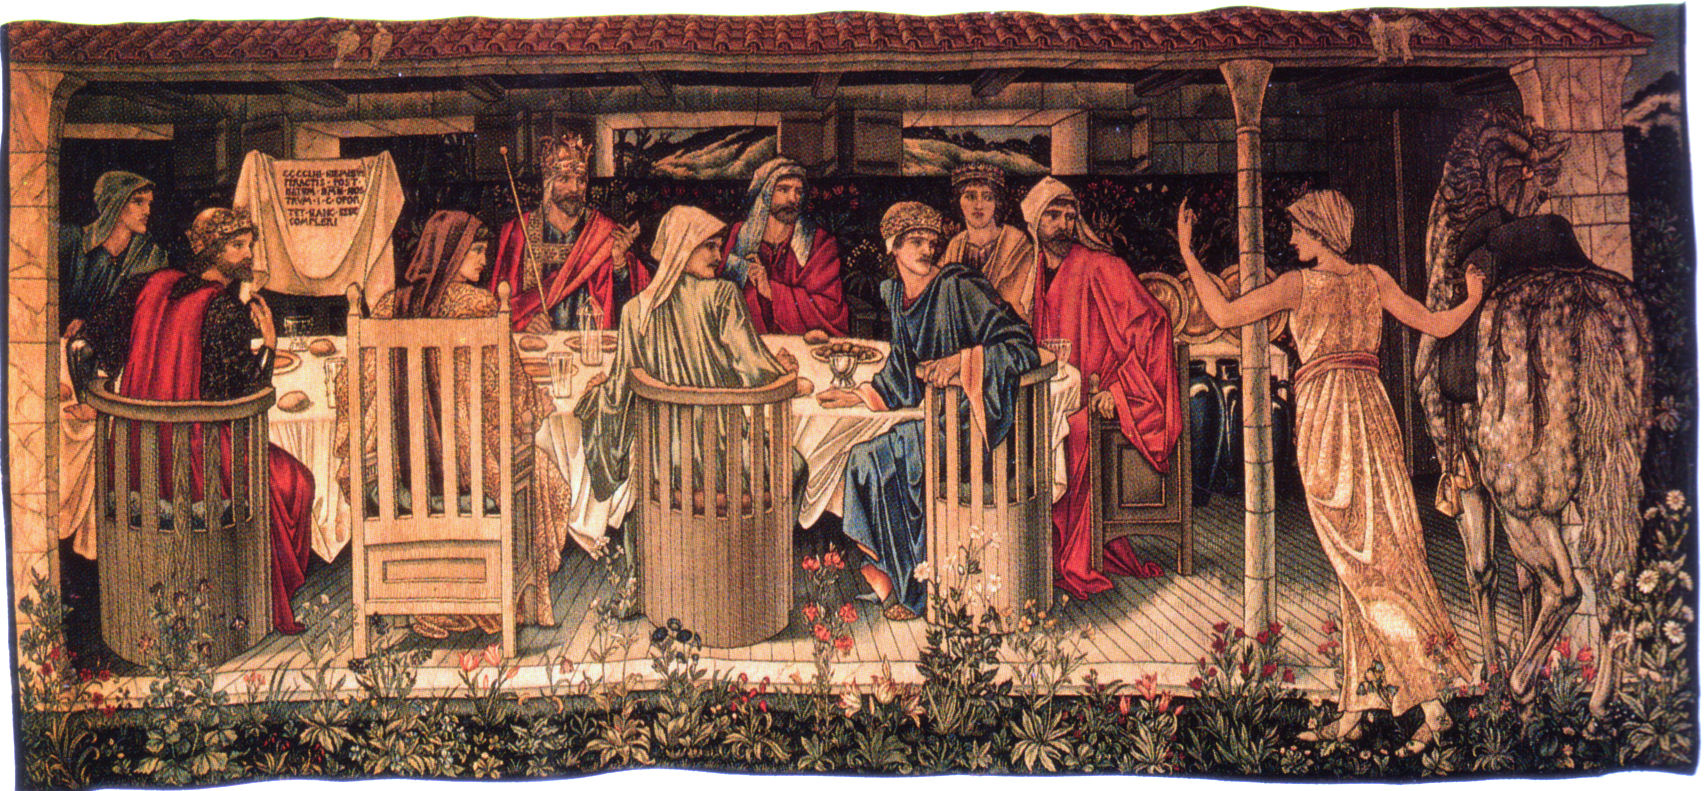
\includegraphics[width=3in]{the_summons}
  \end{center}

  \footnotetext{\textit{The Summons}.The Holy Grail tapestries by Morris \& Co.
    Birmingham Museum and Art Gallery}
\end{frame}

%%%%%%%%%% Statement %%%%%%%%%%%
\begin{frame}
  \frametitle{Tianyu's Thesis Statement}

  \vspace{10pt}
  \begin{center}
  \fbox{
	  \parbox{0.9\linewidth}{\Large It \textit{is possible} to
      design a gradual IFC programming language that satisfies both
      noninterference and the gradual guarantee while supporting type-based
      reasoning, by excluding the unknown label \unk from runtime security
      labels and using security coercions to represent casts.} }
  \end{center}
\end{frame}

%%%%%%%%%% Road Map %%%%%%%%%%%
\begin{frame}
  \frametitle{Road Map}

  \begin{itemize}
  \item[\ding{43}] Background
    \begin{itemize}
    \item Explicit flow and implicit flow
    \item Information flow control (IFC): static, dynamic, and gradual
    \item The gradual guarantee and its tension with IFC
    \item Source of the tension: including \unk in runtime labels
    \end{itemize}
  \item \Surface: a gradual IFC calculus
    \begin{itemize}
      \item \Surface enforces IFC while satisfying gradual guarantee
      \item \Surface supports type-based reasoning (free theorems)
    \end{itemize}
  \item Technical development
    \begin{itemize}
      \item Formal definition of \Surface
      \item Coercion calculi for IFC
      \item The IFC cast calculus \CC
    \end{itemize}
  \item Meta-theoretic results
    \begin{itemize}
      \item Type safety for \Surface
      \item Gradual guarantee for \Surface
      \item Noninterference for \Surface
    \end{itemize}
  \end{itemize}
\end{frame}

%%%%%%%%%% Explicit Information Flow %%%%%%%%%%%
\begin{frame}[fragile]
  \frametitle{Explicit Information Flow}

  Can we infer output from input in the following program?


\begin{lstlisting}[autogobble,numbers=none,xleftmargin=.2\textwidth,xrightmargin=.2\textwidth]
let input = private-input () in
  publish (¬ input)
\end{lstlisting}


\onslide<2-> {
  \begin{itemize}
  \item[\yes] Yes!
  \item Witness at least two executions
  \item Output is the negation of input
  \item \hl{Explicit flow}
  \end{itemize}
}

\end{frame}

%%%%%%%%%% Implicit Information Flow %%%%%%%%%%%
\begin{frame}[fragile]
  \frametitle{Implicit Information Flow}

  Can we infer output from input in the following program?


\begin{lstlisting}[autogobble,numbers=none,xleftmargin=.05\textwidth]
  let input = private-input () in
      publish (if input then false else true)
\end{lstlisting}

\onslide<2-> {
\begin{itemize}
  \item[\yes] Also yes
  \item Again, output is the negation of input
  \item \hl{Implicit flow:} input influences output through \textit{branching}
\end{itemize}
}

\end{frame}

%%%%%%%%%% IFC %%%%%%%%%%%
\begin{frame}
  \frametitle{Information-Flow Control (IFC)}

  \begin{itemize}
  \item Ensures that information transfers adhere to a security policy
    \item For example, \high input must not flow to \low output
    \item Propagate and check the security labels
    \item IFC in PL
      \(
      \left\{
      \begin{minipage}[c]{0.75\linewidth}
      \item[] \bluetext{\Huge static} using a type system
      \item[] \redtext{\Huge dynamic} using runtime monitoring
      \end{minipage}
      \right.
      \)
  \end{itemize}

\end{frame}

%%%%%%%%%% Static IFC, Explicit Flow %%%%%%%%%%%
\begin{frame}[containsverbatim]
  \frametitle{\bluetext{Static IFC} Accepts \textcolor{Green}{Legal} Explicit Flow}

  (Static IFC using a type system)
  \begin{lstlisting}[mathescape,autogobble,xleftmargin=.15\textwidth,xrightmargin=.15\textwidth]
    let fconst = λ b : $\Bool_{\high}$. false in
    let input  = private-input () in
    let result = fconst input in
      publish result
  \end{lstlisting}

  \begin{itemize}
  \item[\yes] \textcolor{Green}{Well-typed}\quad~and~\quad
    \textcolor{Green}{runs successfully} to \texttt{unit}
  \item Why? The return value of \texttt{fconst} is
    \(
    \left\{
    \begin{minipage}[c]{0.3\linewidth}
    \item[] always \texttt{false}
    \item[] of \low-security
    \end{minipage}
    \right.
    \)
  \item Accepted by type-checker. No runtime check
  \end{itemize}

  \footnotetext{\texttt{private-input : $\Unit_{\low}$ → $\Bool_{\high}$}~and~\texttt{publish : $\Bool_{\low}$ → $\Unit_{\low}$}}
\end{frame}


\begin{frame}[containsverbatim]
  \frametitle{\bluetext{Static IFC} Rejects \textcolor{Red}{Illegal} Explicit Flow}

  (Replace \texttt{fconst} with \texttt{flip})
  \begin{lstlisting}[mathescape,autogobble,xleftmargin=.1\textwidth]
    let flip   = λ b : $\highlightblue{\Bool_{\low}}$. ¬ b in
    let input  = private-input () in
    let result = flip input in  $\graytext{\text{// compilation error}}$
      publish result
  \end{lstlisting}
  \vspace{15pt}

  \begin{itemize}
  \item[\no] \textcolor{Red}{Ill-typed.} Illegal explicit flow:
  \begin{itemize}
  \item input is \high
  \item \texttt{flip} expects \low argument
  \end{itemize}
  \item Rejected by type-checker. Again no runtime check
  \end{itemize}
\end{frame}

%%%%%%%%%% Dynamic IFC, Explicit Flow %%%%%%%%%%%
\begin{frame}[containsverbatim]
  \frametitle{\redtext{Dynamic} Enforcement of Explicit Flow}

  (Revisit \texttt{flip} with dynamic IFC)
  \begin{lstlisting}[mathescape,autogobble,xleftmargin=.15\textwidth,xrightmargin=.15\textwidth]
    let flip    = λ b. ¬ b in
    let input   = private-input () in
    let result  = flip input in
      publish result    $\graytext{\text{// runtime error}}$
  \end{lstlisting}

  \begin{itemize}
  \item[\no] \textcolor{Red}{Errors} at runtime (regardless of input)
  \item \redtext{A runtime check} happens before calling \texttt{publish}
  \end{itemize}

  In dynamic IFC, runtime values are tagged with their security level. The
  labels can originate from
  \begin{itemize}
  \item primitive operations
  \item annotations on literals
  \item the security level of the execution context
  \end{itemize}

\end{frame}

%%%%%%%%%% Static IFC, Implicit Flow %%%%%%%%%%%
\begin{frame}[containsverbatim]
  \frametitle{\bluetext{Static} Enforcement of Implicit Flow}

  (Different behavior in different branches)
  \begin{lstlisting}[mathescape,autogobble,xleftmargin=.1\textwidth]
    let flip : $\Bool_{\high}$ → $\highlightblue{\Bool_{\low}}$ =
        λ b : $\Bool_{\high}$. $\highlightred{\text{if b then false else true}}$ in
    let input  = private-input () in
    let result = flip input in
      publish result
  \end{lstlisting}

  \begin{itemize}
  \item[\no] \textcolor{Red}{Ill-typed}
  \item Security label on the type of \texttt{if} is the join (least upper
    bound) of its branches (\low) and the branch condition (\high).
  \item Rejected by type-checker. No runtime check
  \end{itemize}

\end{frame}

%%%%%%%%%% Dynamic IFC, Implicit Flow %%%%%%%%%%%
\begin{frame}[containsverbatim]
  \frametitle{\redtext{Dynamic} Enforcement of Implicit Flow}

  (Enforcing implicit flow with dynamic IFC)
  \begin{lstlisting}[mathescape,autogobble,xleftmargin=20pt]
    let flip   = λ b. if b then false else true in
    let input  = private-input () in
    let result = flip input in
      publish result
  \end{lstlisting}

  \begin{itemize}
  \item[\no] \textcolor{Red}{Errors} at runtime (regardless of input)
  \item \texttt{flip} produces a \high value because of \high branch condition
  \item A runtime check happens before calling \texttt{publish}
  \item Illegal implicit flow ruled out \redtext{at runtime}
  \end{itemize}

\end{frame}

\begin{frame}
  \frametitle{Static IFC Is Hard to Use}
  \begin{quote}
    \large
    ``Another myth spread by security researchers is that the planet Earth
    contains more than six programmers who can correctly use security labels and
    information flow control (IFC).''
    \footnote{James Mickens.
    \href{https://scholar.harvard.edu/files/mickens/files/thisworldofours.pdf}{\textit{This
        World of Ours.}} Usenix ;login: 2014}
  \end{quote}
\end{frame}

\begin{frame}
  \frametitle{\purpletext{Gradual IFC} Comes to the Rescue!}

  \begin{tikzpicture}[scale=0.8]
    \draw[loosely dotted,ultra thick,Plum] (1,4)--(4,1);
    \draw[->,ultra thick] (0,0)--(5,0) node[right]{\redtext{speed of development}};
    \draw[->,ultra thick] (0,0)--(0,5) node[above]{\bluetext{performance}};
    \filldraw[NavyBlue] (1,4) circle (2pt) node[anchor=west]{\bluetext{static}};
    \filldraw[Maroon] (4,1) circle (2pt) node[anchor=west]{\redtext{dynamic}};
    \filldraw[Plum] (3,3) circle (2pt) node[anchor=west]{\purpletext{gradual}};
  \end{tikzpicture}

  Principle of Locality: 90\% of execution time in 10\% of the
  code \footnote{Dr. Ranjani Parthasarathi.
  \href{https://www.cs.umd.edu/~meesh/411/CA-online/index.html}{\textit{Computer
      Architecture: Engineering And Technology}}}

  In \purpletext{gradual IFC}, static type information is optional:
  \begin{itemize}
    \footnotesize
    \item Go static in parts of the application where performance matters
    \item Go dynamic when performance matters less, and ease-of-use matters more
  \end{itemize}

\end{frame}

%%%%%%%%%% Gradual IFC %%%%%%%%%%%
\begin{frame}[containsverbatim]
  \frametitle{\purpletext{Gradual Typing} Bridges Static and Dynamic IFC}

  Partially-annotated \texttt{flip}:
  \begin{lstlisting}[mathescape,autogobble,xleftmargin=20pt]
    let flip : $\highlightred{\Bool_{\unk}}$ → $\highlightblue{\Bool_{\low}}$ =
        λ b : $\highlightred{\Bool_{\unk}}$. if b then false else true in
    let input  = private-input () in
    let result = flip input in
      publish result
  \end{lstlisting}

  \begin{itemize}
  \item \textcolor{Green}{Well-typed}\quad~but~\quad\textcolor{Red}{errors at runtime}
  \item Checking happens on the boundaries between static and dynamic fragments
  \item The information flow violation is detected earlier than the dynamic
    version, as \texttt{flip} returns
  \end{itemize}

\end{frame}

%%%%%%%%%% Gradual Guarantee %%%%%%%%%%%
\begin{frame}[containsverbatim]
  \frametitle{The Gradual Guarantee}

  \begin{minipage}{0.3\textwidth}
    \redtext{\footnotesize less precise}
  \begin{lstlisting}[mathescape,autogobble,basicstyle=\tiny\ttfamily,numbers=none]
    let f : $\highlightred{\Bool_{\unk}}$→$\highlightred{\Bool_{\unk}}$ =
        λ b : $\highlightred{\Bool_{\unk}}$. true in
    let i = private-input () in
    let result = f i in
      publish result
  \end{lstlisting}
  \end{minipage}
  {\tiny $\sqsubseteq~$}
  \begin{minipage}{0.3\textwidth}
    \phantom{middling precise}
  \begin{lstlisting}[mathescape,autogobble,basicstyle=\tiny\ttfamily,numbers=none]
      let f : $\highlightred{\Bool_{\unk}}$→$\highlightblue{\Bool_{\low}}$ =
          λ b : $\highlightred{\Bool_{\unk}}$. true in
      let i = private-input () in
      let result = f i in
        publish result
  \end{lstlisting}
  \end{minipage}
  {\tiny $\sqsubseteq~$}
  \begin{minipage}{0.3\textwidth}
    \bluetext{\footnotesize more precise}
  \begin{lstlisting}[mathescape,autogobble,basicstyle=\tiny\ttfamily,numbers=none]
      let f : $\highlightblue{\Bool_{\high}}$→$\highlightblue{\Bool_{\low}}$ =
          λ b : $\highlightblue{\Bool_{\high}}$. true in
      let i = private-input () in
      let result = f i in
        publish result
  \end{lstlisting}
  \end{minipage}

  \vspace{20pt}

  \begin{itemize}
  \item In the absense of errors, adding or removing security annotations does
    not change the result of the program
  \item Adding security annotations may trigger errors
  \item Removing security annotations may not trigger errors
  \end{itemize}
\end{frame}

%%%%%%%%%% Static IFC Through Heap %%%%%%%%%%%
\begin{frame}[containsverbatim]
  \frametitle{\bluetext{Static} Enforcement of Flows Through \\ Mutable References}

  \vspace{-15pt}
  \begin{lstlisting}[mathescape,autogobble,xleftmargin=.2\textwidth,xrightmargin=.1\textwidth]
    let a     = ref $\low$ true in
    let input = private_input () in
    if input then
        a := false
    else
        a := true
    publish (! a)
  \end{lstlisting}

  \begin{itemize}
  \item The reference has type $\Refer{(\Bool_{\low})}$. It points to a low memory location
  \item The type of the branch condition is $\Bool_{\high}$
  \item[\no] \st{Writing to low memory under a high branch condition}
  \end{itemize}

\end{frame}

%%%%%%%%%% Dynamic IFC Through Heap %%%%%%%%%%%
\begin{frame}[containsverbatim]
  \frametitle{\redtext{Dynamic} Enforcement of Flows Through \\ Mutable References}

  \vspace{-15pt}
  \begin{lstlisting}[mathescape,autogobble,xleftmargin=.2\textwidth,xrightmargin=.1\textwidth]
    let a     = ref $\low$ true in
    let input = private_input () in
    if input then
        a := false
    else
        a := true
    publish (! a)
  \end{lstlisting}

  The assignments fail at runtime because the no-sensitive-upgrade (NSU)
  mechanism \footnote{Austin and Flanagan.
  \href{https://doi.org/10.1145/1554339.1554353}{\textit{Efficient
      purely-dynamic information flow analysis.}} PLAS 2009.} prevents writing
  to a \low security pointer in a \high security branch.

\end{frame}

%%%%%%%%%% Counterexample of GG %%%%%%%%%%%
\begin{frame}[containsverbatim]
  \frametitle{Counterexample of Gradual Guarantee in \GSLRef}

  \begin{multicols}{2}
    \noindent
    \redtext{less precise}
    \begin{lstlisting}[mathescape,autogobble,basicstyle=\footnotesize\ttfamily]
        let x = private-input () in
        let a = ref $\unk$ $\true_{\unk}$ in
        if x then (a := $\false_{\high}$)
             else ()
    \end{lstlisting}
    \columnbreak
    \bluetext{more precise}
    \begin{lstlisting}[mathescape,autogobble,numbers=none,basicstyle=\footnotesize\ttfamily]
      let x = private-input () in
      let a = ref $\high$ $\true_{\high}$ in
      if x then (a := $\false_{\high}$)
           else ()
    \end{lstlisting}
  \end{multicols}

  \begin{itemize}
  \item[\yes] The \bluetext{more precise} program (right) runs successfully
  \item[\no] But the \redtext{less precise} version (left) errors in
    \GSLRef\footnote{Toro, Garcia, Tanter.
    \href{https://doi.org/10.1145/3229061}{\textit{Type-Driven Gradual Security
        with References.}} TOPLAS 2018.}
  \item The assignment fails because it is in a high-security branch and \GSLRef
    conservatively treats the reference's label ($\unk$) as if it were $\low$
  \end{itemize}

\end{frame}

%%%%%%%%%% No `Dyn` in Runtime Labels %%%%%%%%%%%
\begin{frame}[containsverbatim]
  \frametitle{But wait... \GSLRef allows $\unk$ labels on values?}

  The counterexample depends on labeling a reference with unknown security (\unk):
  \vspace{5pt}
  \begin{lstlisting}[mathescape,autogobble,xleftmargin=.2\textwidth,xrightmargin=.2\textwidth]
    let x = private-input () in
    let a = ref $\unk$ $\true_{\unk}$ in
    if x then (a := $\false_{\high}$)
         else ()
  \end{lstlisting}
  \vspace{5pt}

  \begin{itemize}
  \item Dynamic IFC languages don't use $\unk$ as a runtime
    security label.
  \item Gradual languages traditionally use $\unk$ for type
    checking, but not for categorizing runtime values.
  \item The inputs to an information flow system are the user's
    choices regarding what data is high or low security.
  \end{itemize}

\end{frame}

%%%%%%%%%% Sources of Tension %%%%%%%%%%%
\begin{frame}
  \frametitle{Sources of the Tension with the Gradual Guarantee}

\begin{table}[tbp]
  \scriptsize
  \centering
  \begin{tabularx}{\textwidth}{X|c|c|c|c|c}
  \hline
  \thead{Lang.} & \thead{Noninter-\\ference} & \thead{Gradual\\Guarantee} &
  \thead{Type-guided \\ classification} & \thead{NSU} & \thead{Runtime \\ security labels} \\
  \hline
  \GSLRef    & \mytikzmark{a}{\yes}  & \cellcolor{Red!10} \mytikzmark{b}{\no} & \yes  & \yes & $\{ \low, \high, \unk \}$ \\[1ex]
  \hline
  GLIO      & \yes & \cellcolor{Green!10} \mytikzmark{c}{\yes} & \mytikzmark{d}{\no}  & \yes & $\{ \low, \high \}$ \\[1ex]
  \hline
  \WHILEG & \yes & \cellcolor{Green!10} \mytikzmark{e}{\yes} & \yes   & \mytikzmark{f}{\no} & $\{ \low, \high, \unk \}$ \\[1ex]
  \hline
  \rowcolor{highlight}
  \purpletext{\Surface (ours)} & \yes & \cellcolor{Green!10} \mytikzmark{g}{\yes} & \yes & \yes & \mytikzmark{h}{$\{ \low, \high \}$} \\[1ex]
  \hline
  \end{tabularx}
\begin{tikzpicture}[overlay, remember picture, yshift=.25\baselineskip, shorten >=.5pt, shorten <=.5pt]
  \draw[dashed,thick] (a) to [bend right=15] (b);
  \draw[dashed,thick] (c) to [bend right=15] (d);
  \draw[dashed,thick] (e) to [bend right=10] (f);
  \draw[thick]        (g) to [bend right=8 ] (h);
\end{tikzpicture}
  \label{tab:cc-features}
\end{table}

Removing \unk from the runtime labels enables the gradual guarantee.

\end{frame}

%%%%%%%%%% Road Map %%%%%%%%%%%
\begin{frame}
  \frametitle{Road Map}

  \begin{itemize}
  \item Background
  \item[\ding{43}] \Surface: a gradual IFC calculus
    \begin{itemize}
      \item \Surface enforces IFC while satisfying gradual guarantee
      \item \Surface supports type-based reasoning (free theorems)
    \end{itemize}
  \item Technical development
  \item Meta-theoretic results
  \end{itemize}
\end{frame}

%%%%%%%%%% Example in LambdaIFCStar %%%%%%%%%%%
\begin{frame}[fragile]
  \frametitle{\Surface Excludes \unk From Runtime Labels}

  \begin{multicols}{2}
    \noindent
    \redtext{less precise}
    \begin{lstlisting}[mathescape,autogobble,basicstyle=\footnotesize\ttfamily]
      let x = private-input () in
      let a : $\highlightred{(\Refer{\Bool_{\unk}})_{\unk}}$ =
          ref $\high$ $\true_{\high}$ in
      if x then (a := $\false_{\high}$)
           else ()
    \end{lstlisting}
    \columnbreak
    \bluetext{more precise}
    \begin{lstlisting}[mathescape,autogobble,numbers=none,basicstyle=\footnotesize\ttfamily]
      let x = private-input () in
      let a : $\highlightblue{(\Refer{\Bool_{\high}})_{\high}}$ =
          ref $\high$ $\true_{\high}$ in
      if x then (a := $\false_{\high}$)
           else ()
    \end{lstlisting}
  \end{multicols}

  \begin{itemize}

  \item[\yes] The \bluetext{more precise} program runs \textcolor{Green}{successfully} to \texttt{unit}
  \item[\yes] The \redtext{less precise} program also runs \textcolor{Green}{successfully} to \texttt{unit}
  \onslide<2-> {
  \item[\yes] \greentext{\Huge Problem solved!}
  }
  \end{itemize}

  \onslide<2> {
  \begin{tikzpicture}[remember picture,overlay]
    \node [anchor=south east] at ([xshift=-30pt, yshift=10pt]current page.south east)
          {
\includegraphics[height=90pt]{yay}};
  \end{tikzpicture}
  }
\end{frame}

%%%%%%%%%% Comparison %%%%%%%%%%%
\begin{frame}[fragile]
  \frametitle{Comparing \Surface With \GSLRef}

  \begin{itemize}
  \item The default security label in \Surface is \low, so the programmer does not
  have to label constants
  \item Remove the labels on constants to obtain the following program, which also
  reduces successfully to unit:
  \end{itemize}

  \begin{lstlisting}[mathescape,autogobble,numbers=none,xleftmargin=.15\textwidth,xrightmargin=.1\textwidth]
    let x = private-input () in
    let a : $(\Refer{\Bool_{\unk}})_{\unk}$ = ref $\highlight{highlight}{\high}$ true in
    if x then (a := false)
         else ()
  \end{lstlisting}

  \begin{center}
  Comparing with the program in \GSLRef, which errors:
  \end{center}
  \begin{lstlisting}[mathescape,autogobble,numbers=none,xleftmargin=.15\textwidth,xrightmargin=.1\textwidth]
    let x = private-input () in
    let a = ref $\highlight{highlight}{\unk}$ $\true_{\unk}$ in
    if x then (a := $\false_{\high}$)
         else ()
  \end{lstlisting}
\end{frame}

%%%%%%%%%%% Type-Based Reasoning %%%%%%%%%%%%
\begin{frame}[containsverbatim]
  \frametitle{Vigilance: Type-Based Reasoning for Explicit Flows}

  Consider the example from Toro et al. [2018]:

  \begin{lstlisting}[mathescape,autogobble]
    let mix : $\Int_{\low}$ → $\Int_{\high}$ → $\Int_{\low}$ =
      λ pub priv .
        if pub < (priv : $\Int_{\unk}$ : $\Int_{\low}$) then 1 else 2 in
    mix 1$_{\low}$ 5$_{\low}$
  \end{lstlisting}

  \bigskip

  \ul{Free theorem:} The \texttt{mix} function either \textcircled{1} returns a
  value that does not depend on \texttt{priv} or \textcircled{2} produces a
  runtime error

  \bigskip

  %% {\footnotesize
  %%   (GLIO: not vigilant $\rightarrow$ does not produce an error
  %%   $\rightarrow$ violates the free theorem)}
  \bigskip

  In \Surface,\quad$\cccast{\key{5}}{\up \seq \highlightred{\inj{\high} \seq \proj{\low}{p}}} \longrightarrow \blame{p}$
\end{frame}

\begin{frame}[containsverbatim]
  \frametitle{Type-Guided Classification: \\ Type-Based Reasoning for Implicit Flows}

  Consider another example from Toro et al. [2018]:
  \begin{lstlisting}[mathescape,autogobble]
    let mix : $\Int_{\low}$ → $\Int_{\unk}$ → $\Int_{\low}$ =
      λ pub priv. if pub < priv then 1 else 2 in
    let smix : $\Int_{\low}$ → $\Int_{\high}$ → $\Int_{\low}$ =
      λ pub priv. mix pub priv in
    smix 1$_{\low}$ 5$_{\low}$
  \end{lstlisting}

  \bigskip

  \ul{Free theorem:} The \texttt{smix} function either \textcircled{1} returns a
  value that does not depend on \texttt{priv} or \textcircled{2}
    produces a runtime error

  %% {\footnotesize
  %%   (GLIO: \textcircled{1} not vigilant \textcircled{2} does not classify values using types
  %%   $\rightarrow$ does not produce an error
  %%   $\rightarrow$ violates the free theorem)}

\end{frame}

\begin{frame}[containsverbatim]

  \frametitle{Type-Based Reasoning for Implicit Flows in \Surface}

  \begin{minipage}{0.5\textwidth}
    \begin{lstlisting}[mathescape,autogobble,basicstyle=\tiny\ttfamily,numbers=none]
      let mix : $\Int_{\low}$ → $\Int_{\unk}$ → $\Int_{\low}$ =
        λ pub priv. if pub < priv then 1 else 2 in
      let smix : $\Int_{\low}$ → $\Int_{\high}$ → $\Int_{\low}$ =
        λ pub priv. mix pub priv in
      smix 1$_{\low}$ 5$_{\low}$
    \end{lstlisting}
  \end{minipage}
  {\tiny $\Rightarrow$~}
  \begin{minipage}{0.45\textwidth}
    \begin{lstlisting}[mathescape,autogobble,basicstyle=\tiny\ttfamily,numbers=none]
      let mix = λ pub priv.
        (if ((pub ⟨$\,\colorbox{highlight}{\inj{\low}}\,$⟩) < priv)
              then (1 ⟨$\,\colorbox{highlight}{\inj{\low}}\,$⟩)
              else (2 ⟨$\,\colorbox{highlight}{\inj{\low}}\,$⟩)) ⟨$\,\colorbox{highlight}{\proj{\low}{p}}\,$⟩ in
      let smix = λ pub priv.
        mix pub (priv ⟨$\,\colorbox{highlight}{\inj{\high}}\,$⟩) in
      smix 1 (5 ⟨$\,\colorbox{highlight}{\up}\,$⟩)
    \end{lstlisting}
  \end{minipage}

  \bigskip

  {\scriptsize
    \begin{align*}
      \longrightarrow^{*} &
      \quad \cccast{\texttt{(if (\cccast{\key{1}}{\inj{\low}} < \cccast{\key{5}}{\up\seq\inj{\high}}) then \cccast{\key{1}}{\inj{\low}}{} else ...)}}{\proj{\low}{p}} \\[1ex]
      \longrightarrow^{*} &
      \quad \cccast{\texttt{(if \colorbox{highlight}{(\cccast{\true}{\up\seq\inj{\high}})} then \cccast{\key{1}}{\inj{\low}}{} else ...)}}{\proj{\low}{p}} \\[1ex]
      \longrightarrow^{*} &
      \quad \cccast{\ccsyntax{(}\ccprot{}{\colorbox{highlight}{\high}}{\ccsyntax{(}\cccast{\key{1}}{\inj{\low}}}{}\ccsyntax{)}\ccsyntax{)}}{\proj{\low}{p}} \\[1ex]
      \longrightarrow^{*} &
      \quad \cccast{\cccast{\key{1}}{\up\seq\highlightred{\inj{\high}}}}{\highlightred{\proj{\low}{p}}} \\
      \longrightarrow^{*} &
      \quad \blame{p}
  \end{align*}}

\end{frame}

%%%%%%%%%% Road Map %%%%%%%%%%%
\begin{frame}
  \frametitle{Road Map}

  \begin{itemize}
  \item Background
  \item \Surface: a gradual IFC calculus
  \item[\ding{43}] Technical development
    \begin{itemize}
    \item Formal definition of \Surface
    \item Coercion calculi for IFC
    \item The IFC cast calculus \CC
    \end{itemize}
  \item Meta-theoretic results
  \end{itemize}
\end{frame}

%%%%%%%%%% Syntax %%%%%%%%%%%
\begin{frame}
  \frametitle{Syntax of \Surface}

  We define a gradual IFC calculus \Surface with mutable references, first-class
  functions, and conditionals. Highlighted security labels default to \low if
  omitted:

  {\small \[
           \begin{array}{rcl}
             \ell & \in & \{\low,\high\}  \\
             g & \in & \{\low,\high,\unk\} \\
             \iota     & ::= & \Unit \MID \Bool \\
             T      & ::= & \iota \MID \Fun{A}{g}{A} \mid \Refer{(T_g)} \\
             A      & ::= & T_g \\
             M & ::=  & x \MID k_{\highlight{highlight}{\ell}} \MID \lam{g}{x}{A}{M}{\highlight{highlight}{\ell}} \MID \app{M}{M}{p} \\
             & \MID & \ifexp{M}{M}{M}{p} \\
             & \MID & \refexp{\highlight{highlight}{\ell}}{M}{p} \MID \deref{M}{p} \MID \assign{M}{M}{p}
           \end{array}
           \]}

  \vspace{10pt}

\end{frame}

\begin{frame}
  \frametitle{Semantics of \Surface}

  The semantics of \Surface is by translation $\mathcal{C}$ to a cast calculus.

  \begin{figure}[tbp]
    \scriptsize
    \raggedright
        \[
          \begin{array}{rcll}
            \text{evaluation result}     & r & ::=  & k \MID \mathit{fun} \MID \mathit{addr} \MID \mathit{diverge} \MID \mathit{stuck}
          \end{array}
        \]
        \fbox{$\mathit{obs}(V)=r$}
        \begin{align*}
          \mathit{obs}(k) =&\, k \\
          \mathit{obs}(\cccast{k}{\bm{c}}) =&\, k \\
          \mathit{obs}(\cclam{x}{N}) =&\, \mathit{fun} \\
          \mathit{obs}(\cccast{(\cclam{x}{N})}{\bm{c}}) =&\, \mathit{fun} \\
          \mathit{obs}(\ccaddr{n}) =&\, \mathit{addr} \\
          \mathit{obs}(\cccast{(\ccaddr{n})}{\bm{c}}) =&\, \mathit{addr}
        \end{align*}
        Let $M$ be a well-typed \Surface term: $(x{:}\Bool_{\high});\low\vdash M :\Bool_{\low}$ \\[2ex]
        \fbox{$\mathit{eval}(M, b)=r$}
        \begin{align*}
          \mathit{eval}(M, b) =&\, \mathit{obs}(V)\;&\text{if}\;(\compile{M})[x:=b] \mid \emptyset \Downarrow V \mid \mu \\
          \mathit{eval}(M, b) =&\, \mathit{diverge} \;&\text{if~}\;(\compile{M})[x:=b] \mid \emptyset \Downarrow \blame{\bl{p}} \mid \mu \\
                                                    & &\text{or}~ (\compile{M})[x:=b] \mid \emptyset \Uparrow \\
          \mathit{eval}(M, b) =&\, \mathit{stuck}\;&\text{otherwise}
        \end{align*}
  \end{figure}

\end{frame}

%%%%%%%%%%% Technical Development %%%%%%%%%%%%%%%
\begin{frame}
  \frametitle{The Cast Calculus \CC}

  The casts in \CC are represented by coercions on types (a la Henglein) and
  coercions on security labels.

  \[
  \footnotesize
  \begin{array}{rcl}
    c     & ::=  & \id{g} \MID \highlight{highlight}{\up} \MID \inj{\ell} \MID \proj{\ell}{p} \MID \bot^{\bl{p}} \\
    \bar{c} & ::=  & \id{g} \MID \bot^{\bl{p}} \MID \bar{c} \seq c \\
    e & ::= & \ell \MID \blame{p} \MID \cccast{e}{\bar{c}} \\
    c_r  & ::=  & \id{\iota} \MID \refco{\bm{c}}{\bm{c}} \MID \left( \funco{\bar{c}}{\bm{c}}{\bm{c}} \right) \\
    \bm{c} & ::= & (\coerc{c_r}{\bar{c}}) \\
    M & ::=  & x \MID k \MID \cclam{x}{M}\MID \cclet{x}{M}{A}{M}  \\
    & \MID & \highlightred{\cccast{M}{\bm{c}}} \\
    & \MID & M \cdot M \MID \highlight{highlight}{M \cdot^{\star} M} \\
    & \MID & \key{if}\,M\,\key{then}\,M\,\key{else}\,M \MID \highlight{highlight}{\key{if}^{\star}\,M\,\key{then}\,M\,\key{else}\,M} \\
    & \MID & \ccref{\ell}{M} \MID \highlightred{\ccrefproj{\ell}{M}{p}} \MID \ccsyntax{!}\,M \MID \highlight{highlight}{\ccsyntax{!}^\star\,M} \\
    & \MID & M\,\ccsyntax{:=}\,M \MID \highlightred{M\,\ccsyntax{:=?}^{\bl{p}}\,M} \\
    & \MID &{\color{gray} \ccaddr{n} \MID \ccprot{e}{\ell}{M}{A} \MID  \blame{p}} \\
  \end{array}
  \]

\end{frame}

%%%%%%%%%% Road Map %%%%%%%%%%%
\begin{frame}
  \frametitle{Road Map}

  \begin{itemize}
  \item Background
  \item \Surface: a gradual IFC calculus
  \item Technical development
  \item[\ding{43}] Meta-theoretic results
    \begin{itemize}
      \item Type safety for \Surface
      \item Gradual guarantee for \Surface
      \item Noninterference for \Surface
    \end{itemize}
  \end{itemize}
\end{frame}

%%%%%%%%%%% Type Safety %%%%%%%%%%%
\begin{frame}

  \begin{figure}[tbp]
    \raggedright
    \fbox{$\vdash r : A$}
    \begin{gather*}
      \small
      \inference{k : \iota}{\vdash k : \iota_{\ell}}
      \qquad
      \inference{}{\vdash \mathit{addr} : (\Refer{A})_{g}}
      \\[1ex]
      \inference{}{\vdash \mathit{fun} : (\Fun{A}{g_2}{B})_{g_1}}
      \qquad
      \inference{}{\vdash \mathit{diverge} : A}
    \end{gather*}
  \end{figure}

  \begin{theorem}[Type safety of \Surface]
    If $M$ is a well-typed \Surface term: $(x{:}\Bool_{\high});\low\vdash M :
    \Bool_{\low}$ and $\mathit{eval}(M,b)=r$ \\ then the evaluation result is
    well-typed $\vdash r : \Bool_{\low}$.
  \end{theorem}
\end{frame}

%%%%%%%%%%% Gradual Guarantee %%%%%%%%%%%
\begin{frame}
  \begin{theorem}[Gradual guarantee for \Surface]
    Suppose $M$ and $M'$ are well-typed \Surface terms:
    \begin{align*}
    (x{:}\Bool_{\high});\low\vdash& M : \Bool_{\low} \\
    (x{:}\Bool_{\high});\low\vdash& M' : \Bool_{\low}
    \end{align*}
    and they are related by precision: $\vdash M \sqsubseteq M'$. If
    \[
    \mathit{eval}(M', b_1)=b_2
    \]
    then
    \[
    \mathit{eval}(M, b_1)=b_2
    \]
  \end{theorem}
\end{frame}

%%%%%%%%%%% Noninterference %%%%%%%%%%
\begin{frame}
  \begin{theorem}[Noninterference for \Surface]
    If $M$ is a well-typed \Surface term: $(x{:}\Bool_{\high});\low\vdash M : \Bool_{\low}$ and
    \[
    \mathit{eval}(M,b_1)=b_1'
    \]
    and
    \[
    \mathit{eval}(M,b_2)=b_2'
    \]
    then $b_1' = b_2'$.
  \end{theorem}
\end{frame}

%%%%%%%%%% The End %%%%%%%%%%%
\begin{frame}
  \frametitle{Conclusion}

  \begin{itemize}
  \item It is possible to satisfy noninterference and the gradual guarantee
    while supporting type-based reasoning.
  \item The security labels on constants and memory locations should default to
    \low or \high so that \unk is not included in runtime security labels.
  \item Security checks can be modeled using coercions.
  \item Show me the code! The Agda mechanization of \Surface is at
    \begin{center}
      \url{https://github.com/Gradual-Typing/LambdaIFCStar}
    \end{center}
  \end{itemize}

\end{frame}

\begin{frame}
  \centering \Huge \bluetext{Thank you! \smiley{}}
\end{frame}

\begin{frame}
  \frametitle{NSU Checking}

  \begin{figure}
    \footnotesize
  \raggedright
  \fbox{\reduce{M}{\mu}{\PC}{N}{\mu'}} \\[3ex]
  \begin{gather*}
  \inference{n \; \mathbf{FreshIn} \; \mu(\ell) & \highlightred{\cccast{\PC}{\unk \Rightarrow^{\bl{p}} \ell} \longrightarrow^{*} \PC'} }
            {\reduce{\ccrefproj{\ell}{V}{p}}{\mu}{\PC}{\ccaddr{n}}{(\mu , \ell \mapsto n \mapsto V)}}
  \\[3ex]
  \inference{\mathbf{NF}\;\bar{c} & \vdash \bm{c} : T_g \Rightarrow S_{\hat{\ell}} & \vdash \bm{d} : S_{\hat{\ell}} \Rightarrow T_g \\ \highlightred{\cccast{(\mathit{stamp!}\;\PC\;|\bar{c}|)}{\unk \Rightarrow^{\bl{p}} \hat{\ell}} \longrightarrow^{*} \PC'} \\ \cccast{V}{\bm{c}} \longrightarrow^{*} W}
            {\reduce{\left(\cccast{\ccaddr{n}}{\coerc{\refco{\bm{c}}{\bm{d}}}{\bar{c}}}\right)\,\ccsyntax{:=}^{\bl{p}}\,V}{\mu}{\PC}{\unit}{[\hat{\ell} \mapsto n \mapsto W] \; \mu}}
  \end{gather*}
  \end{figure}
\end{frame}

\begin{frame}
  \frametitle{Aligning Less Precise With More Precise}
  Consider the following \Surface terms related by precision:
  \[
  \true_{\low} : \Bool_{\unk} : \Bool_{\unk} \qquad\text{ and }\qquad
  \true_{\low} : \Bool_{\high} : \Bool_{\unk}
  \]
  We need to show the two coercion sequences are related:
  \[
  \vdash \id{\low} \seq \inj{\low} \sqsubseteq \id{\low} \seq \highlight{highlight}{\up} \seq \inj{\high}
  \]
\end{frame}

\end{document}
